%!TEX root = ../main.tex
%%%%%%%%%%%%%%%%%%%%%%%%%%%%%%%%%%
% Links:
%
% Difficulty:
% Companies: 
%%%%%%%%%%%%%%%%%%%%%%%%%%%%%%%%%%


%\begin{figure}
%	\centering
%	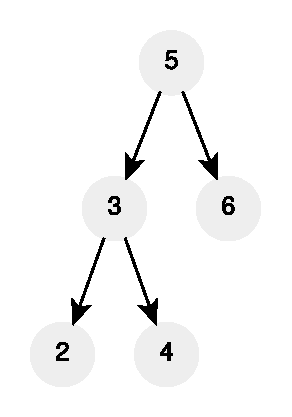
\includegraphics[width=\textwidth]{sources/find_repeated_number_n_divided_3_times/images/example1}
%	\caption[Sample short cpation]{Sample Caption}.
%	\label{fig:find_repeated_number_n_divided_3_times:example1}
%\end{figure}

\section{Find the element repeated $\frac{n}{k}$ times.}
\label{ch:find_repeated_number_n_divided_3_times}
%\section*{Introduction}

\begin{exercise}
\label{example:find_repeated_number_n_divided_3_times:exercice1}
Write a function that, given an array $A$ of $n$ integers and an integer $k$,
returns any of its element that occurs more than  $\frac{n}{k}$.
If such an element does not exists the function returns $-1$.


	%example1
	\begin{example}
		\label{example:find_repeated_number_n_divided_3_times:example1}
		\hfill \\
		Given $A=\{1,2,1,3,1\}$ and $k=3$, the function return $1$ as it occurs $3 > \Big\lfloor\frac{|A|}{3}\Big\rfloor =2$ times.
	\end{example}

	%example2
	%\begin{example}
	%	\label{example:find_repeated_number_n_divided_3_times:example2}
	%	\hfill \\
	%\end{example}
\end{exercise}

%\section{Clarification Questions}
%\begin{QandA}
	%\item 
	%\begin{answered}
		%\textit{}
	%\end{answered}	
%\end{QandA}


\subsection{Boyer-Moore algorithm extended}
\label{find_repeated_number_n_divided_3_times:sec:boyer_moore_extended}
Solution approach:

if you have three distinct elements in the array the solution does not change. You can ignore all three of them.

Therefore, just keep track of the frequencies of two elements.
When you process a new element you can do the following:

1. if you do not have three elements in the frequency list. add it with frequency onesid
2. if the element is equal to another element in the list. increase its frequency
3. if it is a new element (not in the list), decrease the frequency of all in the list by one. Remove any element with frequency zero.
\begin{minipage}{\linewidth}
	\lstinputlisting[language=c++, caption={Sample Caption},label=list:find_repeated_number_n_divided_3_times]{sources/find_repeated_number_n_divided_3_times/find_repeated_number_n_divided_3_times_solution1.cpp}
\end{minipage}